
%(BEGIN_QUESTION)
% Copyright 2009, Tony R. Kuphaldt, released under the Creative Commons Attribution License (v 1.0)
% This means you may do almost anything with this work of mine, so long as you give me proper credit

Here is an oscilloscope's view of an eight-bit data stream sent asynchronously with no parity bit and two stop bits (``8-N-2''), using {\it NRZ} (Non-Return to Zero) encoding.  ``Non-Return to Zero'' is a fancy way of saying a constant ``high'' voltage represents consecutive {\it spaces} and a constant ``low'' voltage represents consecutive {\it marks} -- the simplest encoding scheme possible: 

$$\includegraphics[width=15.5cm]{i02365x01.eps}$$

Identify the following from this waveform:

\begin{itemize}
\item{} All ``Mark'' and ``Space'' states
\item{} The location and state of the {\it start bit}
\item{} The eight-bit binary data represented by this waveform
\item{} The location and state of the {\it stop bits}
\item{} The default ``idle'' state between serial data packets
\end{itemize}

\vskip 20pt \vbox{\hrule \hbox{\strut \vrule{} {\bf Suggestions for Socratic discussion} \vrule} \hrule}

\begin{itemize}
\item{} Explain why it is critically important that we know in advance this is an {\it eight-bit} data frame.
\item{} In this particular example, is the number of stop bits significant?  Why or why not?
\item{} What would be different in this waveform if the frame format were 8-E-2 rather than 8-N-2?
\item{} What would be different in this waveform if the frame format were 8-O-2 rather than 8-N-2?
\end{itemize}

\underbar{file i02365}
%(END_QUESTION)





%(BEGIN_ANSWER)

$$\includegraphics[width=15.5cm]{i02365x02.eps}$$

It is common in NRZ encoding schemes to transmit the LSB first and the MSB last, so the binary value represented by this waveform is {\tt 01011001}.

%(END_ANSWER)





%(BEGIN_NOTES)

With both EIA/TIA-422 and EIA/TIA-485, a negative $V_{AB}$ (terminal A negative and terminal B positive) defines the ``1'' or {\it mark} state.  This is also the default ``idle'' state when the line is not in communication, and it is also called the ``off'' state here.  Conversely, a positive $V_{AB}$ (terminal A positive and terminal B negative) defines the ``0'' or {\it space} state.  

However, terminal A is sometimes labeled ($-$) and terminal B labeled (+) in respect of the default (idle) state, also called ``1'' or mark.  So, if an isolated-input oscilloscope were connected with the probe tip to (+) and the reference clip to ($-$), the waveform as shown would be upside-down.  Clear as mud, right?

%INDEX% Networking, serial data: asynchronous data format
%INDEX% Networking, serial data: start bit
%INDEX% Networking, serial data: stop bit

%(END_NOTES)


